\documentclass[manuscript,review]{acmart}
\usepackage{enumitem} %List type works
\usepackage{lipsum}%for lipsum works
\usepackage{wrapfig}% for wrapped figure
\usepackage{subcaption}%for sub figures
\usepackage{float}
\usepackage{algorithm}
\usepackage{algpseudocode}
\usepackage{booktabs}
\usepackage{multirow}
% Core packages
\usepackage{amsmath,amssymb}
\usepackage{tikz-cd}
\usepackage{multicol}
\usepackage{listings}
\usepackage{tcolorbox}
\tcbuselibrary{listings}

% Suppress ACM boilerplate/copyright block since this is a reformatted preprint
\renewcommand\footnotetextcopyrightpermission[1]{}
\pagestyle{plain}
 

\lstdefinelanguage{SQLLLM}{
  morekeywords={SELECT,FROM,WHERE,AS},
  sensitive=false,
  morestring=[b]',
  morecomment=[l]{--}
}

\lstdefinestyle{sqlstyle}{
  language=SQLLLM,
  basicstyle=\ttfamily\small,
  keywordstyle=\color{green}\bfseries,
  stringstyle=\color{red},
  showstringspaces=false,
  breaklines=true,
  columns=fullflexible
}
% Paragraphs
\setlength{\parindent}{0pt}
\setlength{\parskip}{0.05em}

\citestyle{acmnumeric}

\title{Optimizing LLM Queries in Relational Data Analytics Workloads}
\author{Shu Liu}
\authornote{Equal contribution.}
\email{lshu@berkeley.edu}
\affiliation{\institution{UC Berkeley}\country{USA}}

\author{Asim Biswal}
\authornotemark[1]
\affiliation{\institution{UC Berkeley}\country{USA}}

\author{Amog Kamsetty}
\affiliation{\institution{UC Berkeley}\country{USA}}

\author{Audrey Cheng}
\affiliation{\institution{UC Berkeley}\country{USA}}

\author{Luis Gaspar Schroeder}
\affiliation{\institution{UC Berkeley}\country{USA}}
\affiliation{\institution{Technical University of Munich}\country{Germany}}

\author{Liana Patel}
\affiliation{\institution{Stanford University}\country{USA}}

\author{Shiyi Cao}
\affiliation{\institution{UC Berkeley}\country{USA}}

\author{Xiangxi Mo}
\affiliation{\institution{UC Berkeley}\country{USA}}

\author{Ion Stoica}
\affiliation{\institution{UC Berkeley}\country{USA}}

\author{Joseph E. Gonzalez}
\affiliation{\institution{UC Berkeley}\country{USA}}

\author{Matei Zaharia}
\affiliation{\institution{UC Berkeley}\country{USA}}

\renewcommand{\shortauthors}{Liu, Biswal, Kamsetty, et al.}

\begin{abstract}
Batch data analytics is a growing application for Large Language Models (LLMs). LLMs enable users to perform a wide range of natural language tasks, such as classification, entity extraction, and translation, over large datasets.However, LLM inference is highly costly and slow: for example, an NVIDIA L4 GPU running Llama3-8B can only process 6 KB of text per second, taking about a day to handle 15 GB of data; processing a similar amount of data costs around \$\~10K on OpenAI's GPT-4o. In this paper, we propose novel techniques that can significantly reduce the cost of LLM calls for relational data analytics workloads. Our key contribution is developing efficient
algorithms for reordering the rows and the fields within each row of an input table to maximize key-value (KV)
cache reuse when performing LLM serving. As such, our approach can be easily applied to existing analytics
systems and serving platforms. Our evaluation shows that our solution can yield up to 3.4× improvement in job
completion time on a benchmark of diverse LLM-based queries using Llama 3 models. Our solution also achieves
a 32\%\ cost savings under OpenAI and Anthropic pricing models.
\end{abstract}
\acmYear{2026}
\acmDOI{10.48550/arXiv.2403.05821}
\acmConference[MLSys'25]{Proceedings of Machine Learning and Systems}{2025}{Santa Clara, CA, USA}
\acmISBN{2403.05821}
\begin{document}
\maketitle
\section{INTRODUCTION}
We start by situating our work in a growing trend: LLMs are no longer just standalone chat tools — we're seeing them get embedded directly into relational analytics pipelines. Major database vendors like AWS Redshift~\cite{aws_redshift_llm}, Databricks~\cite{databricks_ai_functions}, and Google BigQuery~\cite{bigquery_llm} have added LLM invocation directly into their SQL APIs, and DataFrame libraries and frameworks~\cite{chase2022langchain,patel2024lotus} have followed suit. This lets us write queries where an LLM is called once per row of a table — for example, to check whether a customer support response actually addressed a user's request — and we expect this kind of usage, spanning classification, entity extraction, summarization, and translation, to keep growing as analysts adopt LLMs for more of their data processing tasks. We refer to this whole class of queries as "LLM queries."

\begin{tcolorbox}[colback=white, colframe=black, boxrule=0.6pt, arc=1pt, left=4pt, right=4pt, top=2pt, bottom=2pt]
\begin{lstlisting}[style=sqlstyle]
SELECT user_id, request,
    support_response,
  LLM('Did {support_response} address
    {request}?', support_response,
    request) AS success
FROM customer_tickets
WHERE support_response <> NULL
\end{lstlisting}
\end{tcolorbox}

The problem we run into is cost and scale. Real-world tables can have millions of rows, and invoking an LLM per row is computationally expensive — we cite the extreme case where a single L4 GPU running Llama3-8B takes roughly a full day to process 15 GB of text, and doing similar work through GPT-4o's API would cost around \$\~10K.

So we turn to a technique the LLM-serving community has been developing: prompt caching~\cite{kwon2023vllm,zheng2023sglang,ye2024cascade,juravsky2024hydragen,gim2024promptcache}, where the attention states (the key-value or "KV" cache)~\cite{vaswani2023attention} for a shared prompt prefix are stored and reused across requests instead of recomputed from scratch. This doesn't just save compute — providers like OpenAI~\cite{openai_pricing}, Anthropic~\cite{anthropic_prompt_caching}, and Google~\cite{gemini_context_caching} now charge substantially less for cached prompt tokens, so better cache reuse directly cuts our costs too.

We observe, however, that just wiring an analytics engine up to an LLM backend that has caching enabled doesn't get us very far, because the requests as generated naturally from a table aren't structured to maximize shared prefixes. Our central insight is that because we're working in a batch setting — the whole table is known ahead of time — we have the freedom to reorder both the rows and the fields within each row before dispatching requests, arranging things so that consecutive requests overlap as much as possible at the start of their prompts.

We frame this as a search problem over an enormous space: for a table with n rows and m fields, there are $n!·(m!)^{n}$ possible orderings. We show that a natural shortcut — applying one fixed field order across the whole table — leaves significant performance on the table, since per-row field reordering can improve our cache hit count by up to a factor of m over any fixed ordering. This motivates the two algorithms we introduce: \textbf{ Prefix Hit Recursion (OPHR)}, which finds the provably best ordering but has exponential runtime, and \textbf{ Greedy Group Recursion (GGR)}, our practical approximation that uses functional dependencies (like primary/foreign key relationships) and table statistics to prune the search space and stay fast even on large tables.

We implement both algorithms on top of Apache Spark~\cite{zaharia2012rdd} with vLLM~\cite{kwon2023vllm} as the serving backend, and since there wasn't an established benchmark for this kind of workload, we build our own — 16 LLM queries spanning selection, projection, multi-step invocations, and retrieval-augmented generation~\cite{lewis2021rag}, run across seven real datasets like Amazon Product Reviews~\cite{he2016ups}, Rotten Tomatoes reviews~\cite{pang2005stars}, and SQuAD~\cite{rajpurkar2016squad}. Across this benchmark, we find our approach delivers 1.5–3.4× speedups in end-to-end query latency and up to 32\% cost savings under real OpenAI and Anthropic pricing, all while preserving the original meaning of the queries.
\section{BACKGROUND AND MOTIVATION}
Before we get into our actual solution, we use this section to build up the technical picture that motivates it — essentially, everything a reader needs to understand why \textit{request reordering} is even a meaningful lever to pull.

We begin by walking through how \textbf{LLM inference} works at a fairly fundamental level, since our optimization depends on understanding where the real costs come from. Modern LLMs are autoregressive Transformer models~\cite{vaswani2023attention}, meaning they generate output one token at a time, and each new token depends on the entire sequence of tokens that came before it. We break inference into two distinct phases: the prefill phase, where the model processes the full input prompt in one shot, and the decoding phase, where it generates the output tokens sequentially. We note that production serving engines — \textbf{ vLLM~\cite{kwon2023vllm}, TGI~\cite{huggingface_tgi}, TensorRT-LLM~\cite{nvidia2023tensorrt}}, and similar systems — try to make this efficient by continuously batching many requests together~\cite{yu2022orca} so the GPU stays busy rather than sitting idle between individual token generations. Even so, we emphasize that inference remains a genuinely expensive operation: all of the intermediate computed state for every token has to be kept in memory as key and value vectors (the \textbf{KV cache}), and depending on model size this can add up quickly — we cite a rough estimate of up to 800KB per token for a 13B-parameter model~\cite{kwon2023vllm}, meaning a fairly ordinary 2,000-token request might require over a gigabyte and a half of GPU memory just to process. Combined with the fact that current hardware tops out around 2,000 tokens per second per GPU, we frame this as a real structural bottleneck for anyone trying to run LLMs at the scale that analytical workloads demand — not a minor inefficiency, but a fundamental limit on how much data can realistically be processed and how much it costs.

From there, we shift to explaining prompt KV caching as the mechanism the broader LLM-serving community has developed to blunt this cost, and the mechanism our own work builds on top of. The underlying idea is fairly intuitive: if two different requests happen to share an identical prefix — the same opening sequence of tokens — then the computation and cached internal state from processing that prefix the first time can simply be reused the second time, rather than recomputed from scratch~\cite{zheng2023sglang}. This means only the portion of the request that's actually new needs fresh computation, which can meaningfully cut both latency and, since major providers now price cached tokens at a discount, monetary cost as well.

Having established both why inference is expensive and how caching helps, we then turn to why we think relational data in particular is such a promising place to apply this idea. We point out that real-world databases are rarely random — they're full of structured repetition. Columnar storage formats like C-Store and Parquet~\cite{stonebraker2018cstore} already lean on repeated values for compression, and a whole family of existing database techniques — run-length encoding~\cite{lemire2011reordering}, correlation and functional-dependency analysis~\cite{dzeroski2003multirelational,ilyas2004cords}, database cracking~\cite{idreos2007cracking}, multi-dimensional clustering~\cite{chen2012multidimensional}, Delta Lake's Z-ordering~\cite{armbrust2020delta} — exist specifically to reorganize data around these repeated values and access patterns. Our observation is that this same underlying repetitiveness, which the database community has spent decades exploiting for other purposes, maps naturally onto the KV-caching opportunity from LLM serving. Because an LLM query in our setting is invoked once per row over a table whose full contents are already known ahead of time — this isn't a live, unpredictable stream of requests — we're not stuck with whatever row and field order the table happens to arrive in. We have the freedom to rearrange both the order of rows and the order of fields within each row before we ever send anything to the model, specifically to maximize how much of each request's beginning overlaps with the one before it. We formalize this goal as maximizing what we call the \textit{prefix hit count}, and this framing is what sets up the concrete reordering algorithms — OPHR and GGR — that we introduce in the sections that follow.
\section{PROBLEM SETUP}
This section introduces the problem setup of maximizing
prefix hits in the prompt cache (Sec~\ref{sec:setup}) and highlights cases
where naive fixed field ordering can result in significantly
lower hit rates (Sec~\ref{sec:case study}).
\subsection{Setup Objective}
\label{sec:setup}
In this section, our goal is to pin down, in precise mathematical terms, exactly what we mean when we talk about "maximizing prefix hits" — because up to this point we've only described the idea informally, and everything we build in the rest of the paper (our \textbf{OPHR} and \textbf{GGR} algorithms) depends on having a rigorous, unambiguous target to optimize against rather than just an intuition. Let's explore an example query:

\begin{tcolorbox}[colback=white, colframe=black, boxrule=0.6pt, arc=1pt, left=4pt, right=4pt, top=2pt, bottom=2pt]
\begin{lstlisting}[style=sqlstyle]
SELECT LLM("Summarize: ",pr.*)
FROM(
    SELECT review,rating,description
    FROM reviews r JOIN product p ON
      r.asin=p.asin         
)AS pr
\end{lstlisting}
\end{tcolorbox}

We start by describing the general shape of the LLM operator we're designing around, since our reordering strategy only makes sense in the context of how these operators are actually invoked. We define it as a generic function that takes in a natural-language prompt template along with a set of fields drawn from a table — this could be an explicit list like ${T.a, T.b, T.c}$, or it could be all fields at once via ${T.*}$. We deliberately keep this design simple, partly because it mirrors how LLM operators are already implemented in real analytics systems and SQL-like APIs, and partly because this simplicity is exactly what gives us the freedom we need: since the operator just consumes a set of fields rather than a fixed positional structure, we're free to dynamically reorder which fields go into a request, and in what sequence, without changing what the query actually computes. We illustrate this with a running example — a query that joins a reviews table with a product table and asks the LLM to summarize each row using the review text, rating, and description fields — just to make the abstraction concrete before diving into the formalism.

From there, we lay out our actual optimization objective. Given a table with n rows and m fields, we're searching for the best possible ordering of both the rows themselves and the fields within each individual row, with the explicit goal of maximizing how much consecutive requests overlap with each other from the very start of the prompt. To reason about this formally, we represent a candidate ordering as a list of tuples: shuffling the list itself changes the order in which rows are sent to the LLM, while shuffling the values within a given tuple changes the order of fields for that particular row — and importantly, we allow this field order to vary independently from row to row, rather than forcing one fixed layout across the whole table.

We then introduce the central metric that everything in the paper builds on: the \textit{prefix hit count}, or \textbf{PHC}. For each row, we compare its field values against the same fields in the immediately preceding row, starting from the first field in the ordering and continuing to check subsequent fields only as long as every value up to that point still matches. A match has to be exact — not a partial overlap or a substring — and the sequence of matches has to be unbroken from the start; the moment we hit a field that doesn't match, the count for that row stops there. Rather than simply counting how many fields matched, we weight each hit by the sum of the squared lengths of the matching values. We do this specifically because token-by-token computation in LLM inference scales roughly quadratically with sequence length, so a longer shared prefix isn't just "slightly better" than a short one — it represents disproportionately more compute that we get to skip, and we want our metric to reflect that real-world cost structure rather than just counting matches naively.

We define the \textit{prefix hit count} (PHC) of $L$ as the number
of consecutive field cell values shared with the previous
row starting from the first cell, summing over all n rows.
Each cell value must exactly match the corresponding cell
of the previous row (cannot be a substring), and cell values
past the first must match consecutively (must be a prefix).
Formally, a cell in the list of tuples is denoted as $L[r][f]$,
indicating the value in tuple r at position f. Then, the PHC
for a list of tuples L with n rows and m fields is given by:
\begin{equation}
\text{PHC}(L) = \sum_{r=1}^{n} hit(L, r)
\end{equation}

Here, the function $hit(L,r)$ represents the \textit{ prefix hit count}
for a single row r in L. For simplicity, we assume that the
input list is sorted. For each row r, the function checks if
the value in each field f matches any previously seen value
in the same field of the previous row $r-1$. If all previ
ous fields match, the hit count is the sum of the squares of
the lengths of the values in those fields until a mismatch occurs. The squared lengths reflect the quadratic complexity of
token processing in LLM inference, where each token com
putation depends on every preceding token and increases
computational cost quadratically with input length.

\begin{equation}
hit(L, r) = \max_{0 \le c < m}
\begin{cases}
\displaystyle\sum_{f=1}^{c} \operatorname{len}(L[r][f])^2 & \text{if } \forall f \le c,\ L[r][f] = L[r-1][f] \\[0.6em]
0 & \text{otherwise}
\end{cases}
\end{equation}

Finally, we introduce two simplifying assumptions that make the problem more tractable without sacrificing much realism. First, we assume that at least one row's worth of data can fit into the KV cache at any given time, since without that baseline assumption there's no meaningful notion of reuse to begin with. Second, we assume that a cache "hit" requires values to match exactly, ruling out partial or substring matches. We defend this second assumption by pointing out that it's not an artificial constraint we're imposing for convenience — exact-value repetition is already a well-established property that real relational databases are built around and actively optimized for, as seen in techniques like run-length encoding~\cite{lemire2011reordering} and in columnar storage systems like C-Store and Parquet~\cite{stonebraker2018cstore}. We're upfront that these are simplifications rather than a perfectly faithful model of every real-world scenario, but we note that this tradeoff pays off: in our later empirical evaluation (Section~\ref{sec:evaluation}), we show that despite these simplifying assumptions, the resulting approach still performs well on real, messy, real-world data.

\begin{figure}[!htbp]
\centering
\begin{subfigure}[b]{0.4\linewidth}
\centering
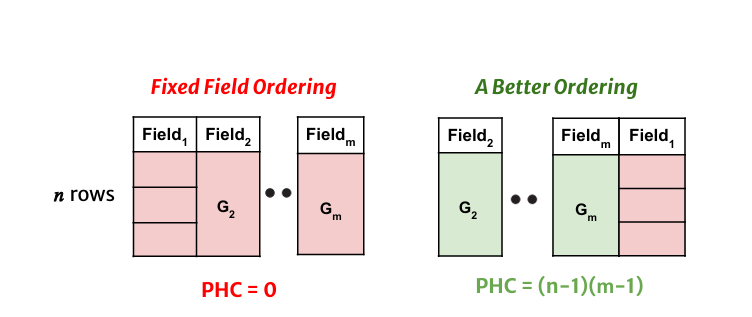
\includegraphics[width=\linewidth]{Images/Distinct Values in the first field.png}
\caption{Distinct Values in the First Field}
\label{fig:Distinct Values in the First Field}
\end{subfigure}
\begin{subfigure}[b]{0.4\linewidth}
\centering
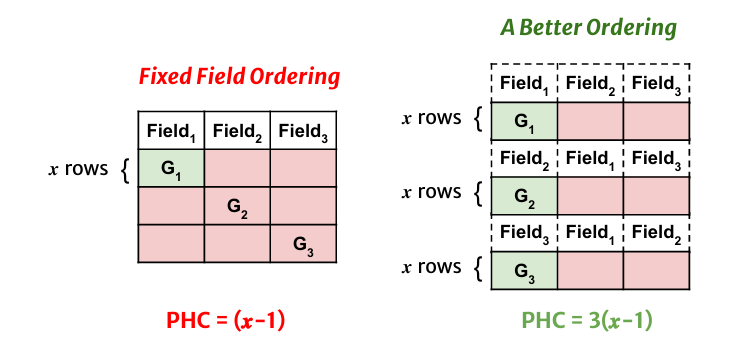
\includegraphics[width=\linewidth]{Images/Group of Identical values in each field ,m=3.png}
\caption{Group of Identical values in each field ,m=3}
\label{fig:Group of Identical values in each field ,m=3}
\end{subfigure}
\caption{\textbf{Case Study of Fixed Field Ordering}: Comparing the PHC of a fixed field ordering to a better ordering in two scenarios. Green
boxes denote cache hits; red boxes indicate cache misses. A box labeled Gi signifies consecutive rows share the same values in Field \textit{i};
otherwise, assume values are distinct. Fig~\ref{fig:Distinct Values in the First Field} shows fixed field ordering can be $(n-1)(m-1)$ worse in terms of PHC compared to an
optimized ordering. Fig~\ref{fig:Group of Identical values in each field ,m=3} shows fixed field ordering can be m times worse in PHC compared to an optimized ordering, where $m = 3$.}
\label{subfig:setup objective}
\end{figure}
\subsection{Case Study: Fixed Field Ordering}
\label{sec:case study}
In this section, our goal is to make the cost of naive, fixed field ordering concrete rather than just asserting it abstractly. Up to this point we've defined PHC formally, but we haven't yet shown why the way relational data is typically laid out — one fixed column order applied uniformly across every row — is actually a real problem worth solving. So we walk through two deliberately simple, worked examples to build intuition before generalizing.

We start with the most extreme case we can construct: a table with n rows and m fields where, for simplicity, every value is exactly one character long. We imagine that the very first field in the table happens to contain completely unique values in every row — something like a timestamp or an ID column, which is extremely common in real data — while every other field repeats the same value across all rows. Because our PHC metric only counts a hit if the match starts from the first field and continues unbroken, this ordering is catastrophic: the moment the first field breaks the streak (which it always does, since every value there is unique), we get zero credit for anything after it, even though the remaining $m-1$ fields are all identical from row to row. So this "obvious," default ordering gives us a PHC of exactly 0. But if we simply move that problematic first field to the end instead, keeping the $m-1$ repetitive fields up front, every row after the first now hits from the very start, and we get a \textbf{PHC} of $(n-1)(m-1)$. We use this to make a first, blunt point: field order alone, without changing a single value in the table, can be the difference between zero cache reuse and substantial reuse.

We then move to a more realistic and more interesting scenario, since real tables rarely have just one messy field — they tend to have this pattern scattered across several fields at once. We imagine a table where each of the $m$ fields has its own "clump" of $x$ consecutive rows sharing an identical value, but these clumps don't line up with each other — they occur in different, non-overlapping stretches of rows depending on which field you look at. We work through a concrete case with 3x rows and 3 fields $(m=3)$. If we insist on one fixed field order applied to the whole table, we can only ever benefit from whichever single field's clump happens to align with our chosen prefix; the other two clumps go completely unused no matter which field we pick, capping our PHC at just $x-1$. But if we're willing to let the field order vary row by row — prioritizing whichever field actually has the matching clump for that particular stretch of rows — we can capture all three clumps instead of just one, tripling our PHC to $3(x-1)$.

We then generalize the intuition from that second example: if this pattern holds across all m fields, with each field containing roughly the same number of these repeating clumps, then dynamic per-row reordering can yield up to an m-fold improvement in PHC compared to any single fixed ordering. To make this tangible in dollar terms rather than just an abstract count, we run through a quick calculation under OpenAI's cache-pricing model (which charges half price for cached tokens): for a nine-field table where the naive fixed ordering only achieves a 10\%\ hit rate ($e.g., \frac{x-1}{n}=10$), optimizing the field order could realistically translate into 42\%\ in actual cost savings.

We use this section, in short, to justify why we don't settle for a simpler, cheaper-to-compute fixed ordering — the case study shows that doing so leaves real, quantifiable performance and money on the table, which is exactly what motivates the two reordering algorithms (\textbf{OPHR} and \textbf{GGR}) we introduce next.
\section{RECURSIVE REQUEST REORDERING}
\label{sec:recursive request reordering}
We now introduce our algorithms that re-arrange fields to
maximize prefix sharing in the KV cache. We present an
optimal recursive reordering algorithm that maximizes PHC
(Sec~\ref{sec:Optimal Prefix Hit Recursion (OPHR)}) and introduce a greedy algorithm that efficiently
approximates the optimal algorithm (Sec~\ref{sec:Greedy Group Recursion (GGR) Algorithm}).
\subsection{Optimal Prefix Hit Recursion (OPHR)}
\label{sec:Optimal Prefix Hit Recursion (OPHR)}
Our Optimal Prefix Hit Maximization (OPHR) algorithm is
a recursive algorithm that finds the $optimal$ PHC for a given
table $T$ by considering all possible ways to split the table
into a group of cells with the same value and two sub-tables.
The algorithm takes as input a table $T$ and computes the
optimal PHC S along with a reordered list of tuples $L$. If
$T$ only has one row or field, OPHR computes PHC and
trivially returns the sorted $T$.

In the recursive case, for each field $c$ in $T$, the algorithm
identifies all distinct values $v$ in the field and the rows $R_{v}$
for which the field value is $v$. For each distinct value $v$, the
table is split into two sub-tables: one of $T$ excluding rows
$R_{v}$ and one of $R_{v}$ excluding field $c$. PHC for the currently
selected value $v$ is calculated as the sum of the PHC of the
sub-tables and the PHC contribution of $v$.

We wrap up our description of OPHR by first noting its practical limitation, then proving it's actually correct.
On the practical side, we're upfront that OPHR, despite giving us the best possible PHC, has exponential complexity in both the number of rows and fields. This comes directly from how the algorithm works: at every step it recursively considers every possible grouping of distinct values across every field, and that combinatorial explosion is exactly what makes it impractical for anything but small tables — which is why we introduce a more efficient, greedy alternative later in Section~\ref{sec:Greedy Group Recursion (GGR) Algorithm}.

On the correctness side, we walk through a formal proof that OPHR genuinely does find the optimal PHC, and we build this proof using mathematical induction, since the algorithm itself is recursive and induction is the natural tool for showing a recursive procedure behaves correctly at every level of recursion. We start with the base cases, which are deliberately simple so there's no ambiguity about what "optimal" means at the smallest scale. If the table has just a single row, there's no previous row to compare against, so there's fundamentally nothing to reuse — the PHC is trivially 0, and no cleverer algorithm could possibly do better. If instead the table has just a single field, the PHC comes down to summing the squared lengths of each repeated value, but discounting the very first time each value appears, since that first occurrence is a genuine cache miss and can't benefit from anything that came before it. These two cases anchor the proof: they establish that the algorithm behaves correctly at the smallest possible inputs, which is the foundation the inductive argument needs to build on. 

\begin{algorithm}[h]
\caption{Greedy Group Recursion (GGR)}
\begin{algorithmic}[1]
\State \textbf{Input:} Table $T$, Functional Dependency $FD$
\State \textbf{Output:} Prefix Hit Count $S$, Reordered List of Tuples $L$

\Function{HitCount}{$v, c, T, FD$}
    \State $R_v \gets \{i \mid T[i,c] = v\}$
    \State $\text{inferred\_cols} \gets \{c' \mid (c,c') \in FD\}$
    \State $\text{tot\_len} = \operatorname{len}(v)^2 + \sum_{c' \in \text{inferred\_cols}} \dfrac{\sum_{r \in R_v} \operatorname{len}(T[r,c'])}{|R_v|}$
    \State \Return $\text{tot\_len} \times (|R_v| - 1),\ [c] + \text{inferred\_cols}$
\EndFunction

\Statex

\Function{GGR}{$T, FD$}
    \If{$|T|_{rows} = 1$}
        \State \Return $0, [T[1]]$
    \EndIf
    \If{$|T|_{cols} = 1$}
        \State $S \gets \sum_{v \in \text{distinct}(T[,1])} \Call{HitCount}{v, 1, T}$
        \State \Return $S, \text{sort}([T[i] \mid i \in 1 \ldots |T|_{rows}])$
    \EndIf
    \State $max\_HC, \hat{v}, \hat{c}, \hat{cols} \gets -1, \text{None}, \text{None}, []$
    \For{$c \in \text{columns}(T),\ v \in \text{distinct}(T[,c])$}
        \State $HC, cols \gets \Call{HitCount}{v, c, T, FD}$
        \If{$HC > max\_HC$}
            \State $max\_HC, \hat{v}, \hat{c}, \hat{cols} = HC, v, c, cols$
        \EndIf
    \EndFor
    \State $R_{\hat{v}} \gets \{i \mid T[i, \hat{c}] = \hat{v}\}$
    \State $A\_HC, L_A \gets \Call{GGR}{T[\text{rows} \setminus R_{\hat{v}}, \text{cols}], FD}$
    \State $B\_HC, L_B \gets \Call{GGR}{T[R_{\hat{v}}, \text{cols} \setminus \hat{cols}], FD}$
    \State $C\_HC, \_ \gets \Call{HitCount}{\hat{v}, \hat{c}, T, FD}$
    \State $S \gets A\_HC + B\_HC + C\_HC$
    \State $L \gets [[\hat{v}] + L_A[i] \mid i \in 1 \ldots |R_{\hat{v}}|] + L_B$
    \State \Return $S, L$
\EndFunction

\Statex

\State \Return \Call{GGR}{$T, FD$}
\end{algorithmic}
\end{algorithm}
For the general, inductive case, we assume as our inductive hypothesis that OPHR already computes the optimal PHC for any table smaller than the one we're currently considering, and our job is to show that this optimality is preserved when we grow the table by one additional row and one additional field. The core mechanism that makes this work is the way OPHR splits the table: for each distinct value appearing in a given field, it divides the table into two sub-tables — one holding all the rows that don't contain that value, and the other holding the rows that do, with that particular field removed from consideration since it's already been accounted for. Because our inductive hypothesis tells us OPHR is already optimal on these two smaller sub-tables, and because the PHC of the full table is exactly equal to the sum of the PHCs of both sub-tables plus whatever contribution came from the value we split on, we've captured the entire picture with nothing left over or double-counted. We emphasize that this splitting step is what makes the whole argument hold together: it keeps each value's contribution to the PHC fully intact rather than letting it get fragmented. If we didn't split the table this way and instead left matching values scattered across non-contiguous groups, we'd risk understating how much reuse is actually achievable. So by consistently splitting along distinct values at every recursive step, OPHR is guaranteed to be considering every genuinely possible configuration, which is exactly why it arrives at the true optimal ordering rather than just a good one.
\begin{figure}[h]
  \centering
  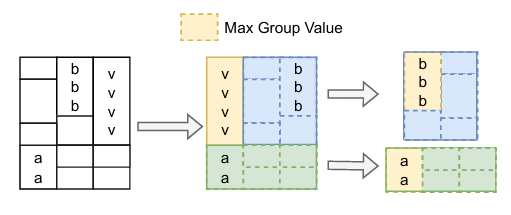
\includegraphics[width=0.8\textwidth]{Images/GGR with group.png}
  \caption{GGR picksthe group with the maximumhit count at each
step and calculates PHC as the sum of PHC of the elected group
values (yellow box), the sub-table T excluding rows $R_{v}$ (green
box), and the sub-table of rows $R_{v}$ excluding the field where the
value is located in (blue box).}
  \label{fig:GGR with group}
\end{figure}
\subsection{Greedy Group Recursion (GGR) Algorithm}
\label{sec:Greedy Group Recursion (GGR) Algorithm}
Since OPHR is computationally infeasible at scale, we use this section to introduce Greedy Group Recursion (GGR), our practical approximation, and to justify why it stays fast while still tracking OPHR's quality closely. The GGR algorithm (Algorithm~1) takes a table $T$ and a set of functional dependencies $FD$ as input, and returns a prefix hit count $S$ together with a reordered list of tuples $L$. It shares the same base cases as OPHR: if $T$ has only one row or one column, GGR falls back to the same trivial computation.

Where GGR diverges from OPHR is in the recursive case. Rather than exhaustively considering every distinct value across every field the way OPHR does, GGR greedily selects a single best candidate value $\hat{v}$ — the one that yields the maximum prefix hit count — at each recursion step (lines 3–8 and 17–23 of the algorithm). It then prioritizes the field $\hat{c}$ that $\hat{v}$ belongs to, splits the table into the group of rows sharing that value versus the rest, and recurses on the two resulting sub-tables (lines 24–26), finally summing the PHC contributions from both sub-tables and from $\hat{v}$ itself (line 28) — structurally mirroring OPHR's recursive decomposition, just without OPHR's exhaustive search.

We explain why this greedy shortcut is so much cheaper: because GGR only ever evaluates one candidate value per step rather than every distinct value in the table, the maximum recursion depth drops to $O(\min(n,m))$, since each recursive call strictly shrinks either the row or column dimension of the table. We do note one caveat, though — at each individual recursive step, the cost of scanning the table to identify distinct values can still be quadratic in table size, so the per-step cost isn't free even though the number of steps is small.
\subsubsection{Functional Dependencies}
\label{FD}
We then explain the first of two mechanisms we use to keep GGR both fast and close to optimal: functional dependencies. We define a functional dependency $FD$ formally as a constraint between two attribute sets $X$ and $Y$ in a relation $R$, where an instance $r$ of $R$ satisfies $X \leftrightarrow Y$ if, for every pair of tuples $t_1, t_2 \in r$: $t_1.X = t_2.X \implies t_1.Y = t_2.Y$, and vice versa. Practically, we use these dependencies to narrow down how many fields GGR has to actively consider at each recursive step: once a value $v$ in field $f$ is chosen for a row, we automatically place every field functionally dependent on $f$ immediately alongside it in the final ordering, rather than treating those dependent fields as separate decisions. We illustrate this with a small example: given a table $R(A, B, C)$ with a functional dependency $A \leftrightarrow C$, once field $A$ has already been placed in the prefix, field $C$ no longer needs to be considered separately in our recursive search, since it's already determined.
\subsubsection{Table Statistics}
\label{Table Stats}
The second mechanism we introduce is an early-stopping strategy driven by table statistics, intended to cut runtime further beyond what functional dependencies alone achieve. We halt recursion either after a fixed recursion depth (separately for row-wise and column-wise recursion) or once a threshold $\text{HITCOUNT}$ score, computed from table statistics, is no longer exceeded. We rely on statistics that are typically already available in databases and analytics systems — cardinality (the number of unique values) and the distribution of value lengths per field. From these, we estimate, for each field $c$:
\[
\text{HITCOUNT}(c) = \operatorname{avg}(\operatorname{len}(c))^2,
\]
which approximates how much that field is likely to contribute to the overall PHC, based on typical value length and frequency. We use this score to prioritize fields more likely to pay off, and once recursion halts early, we fall back to a fixed field ordering for the remaining sub-tables based on these same statistics — letting GGR skip further scanning and recursion on data where it's unlikely to be worthwhile.
\subsubsection{Achieving Optimal PHC}
\label{Optimal PHC}
Finally, we address the natural question of when our greedy approximation actually matches OPHR's true optimum rather than just approximating it. We note that GGR trivially matches OPHR whenever the table has only one row or one field, since both algorithms reduce to the same base case. More interestingly, we show that GGR can also reach the true optimum whenever the functional dependencies available are accurate and span all fields in the table — for instance, if a single field $A$ functionally determines every other field, GGR's accumulated $\text{HITCOUNT}$ score naturally causes it to prioritize groups of values in $A$ first, capturing the important correlations early and yielding the same reordering OPHR would find. We're upfront about where this breaks down, though: when multiple fields tie on $\text{HITCOUNT}$, GGR has no mechanism to break the tie the way OPHR's exhaustive search can, so it may settle for a suboptimal choice in those cases. 
\section{IMPLEMENTATION}
\label{sec:implementation}
In this section, we step back from the algorithms themselves and describe how we actually built and deployed them. We implemented both OPHR and GGR in roughly 1.3 thousand lines of Python, and we chose to evaluate everything on top of PySpark~\cite{armbrust2015spark}, which itself sits on Apache Spark~\cite{zaharia2012rdd} — a large-scale data processing engine we picked specifically because it's so widely used in industry, which makes our results more representative of how these techniques would actually get adopted in practice rather than being tied to some niche or custom-built system.
We explain that the actual LLM invocation is handled by what we call the LLM operator, which we implement as a user-defined function (UDF) inside PySpark — this is the piece that calls out to a configurable LLM endpoint to run inference. This operator takes in a system prompt, a query prompt, and a single row of table data as its inputs, and critically, the order in which the row's fields and the row itself get passed in isn't arbitrary — it's determined directly by whatever ordering our GGR (or OPHR) reordering function computed beforehand. So the reordering algorithm and the actual LLM-calling operator are tightly coupled: one feeds directly into the other.
\section{EVALUATION}
\label{sec:evaluation}
In this section, we evaluate the effectiveness of our opti
mizations within a constructed benchmark suite of queries.
We aim to answer the following questions:
\begin{enumerate}
\item How does our request reordering optimization impact
query latency and costs across different LLM query
types and datasets?
\item How does the request reordering algorithm influence
LLM accuracy for different models? 
\item What is our algorithm solver time, and how does that
compare to end-to-end query latency?
\end{enumerate}
\subsection{Evaluation Benchmark}
\label{Evaluation Benchmark}
Given the lack of standard benchmarks for LLM queries,
we construct a benchmark suite to represent real-world data
retrieval and processing tasks (Sec~\ref{Dataset}). We define a range
of query types (Sec~\ref{LLM queries}) over datasets from various sources
to assess the impact of LLMs in relational analytics.
\textit{\subsubsection{Datasets}}
\label{Dataset}
\begin{table}[H]
\centering
\begin{tabular}{lccccc}
\toprule
Dataset & $n_{\text{rows}}$ & $n_{\text{fields}}$ & input$_{\text{avg}}$ & output$_{\text{avg}}$ & Query Type \\
\midrule
Movies & 15000 & 8 & 276 & \{2, 29, 16, 2\} & T1-T4 \\
Products & 14890 & 8 & 377 & \{3, 107, 62, 2\} & T1-T4 \\
BIRD & 14920 & 4 & 765 & \{2, 43\} & T1, T2 \\
PDMX & 10000 & 57 & 738 & \{2, 72\} & T1, T2 \\
Beer & 28479 & 8 & 156 & \{2, 38\} & T1, T2 \\
SQuAD & 22665 & 5 & 1047 & 11 & T5 \\
FEVER & 19929 & 5 & 1302 & 3 & T5 \\
\bottomrule
\end{tabular}
\caption{Datasets: $n_{\text{rows}}$ and $n_{\text{fields}}$ denote the number of rows and
fields, respectively. input$_{\text{avg}}$ and output$_{\text{avg}}$ represent average input
and output token lengths. Query Type is detailed in Sec 6.1.2.
Since input$_{\text{avg}}$ remains consistent across query types, we report a
single overall average, while output$_{\text{avg}}$ varies, with each bracketed
value corresponding to a specific query type.}
\label{tab:datasets}
\end{table}
We build our benchmark on seven widely-used datasets spanning recommendation and NLP tasks — Rotten Tomatoes movie reviews~\cite{pang2005stars}, Amazon product reviews~\cite{he2016ups}, BIRD~\cite{li2024bird}, PDMX~\cite{long2024pdmx}, RateBeer reviews~\cite{mcauley2012ratebeer}, SQuAD~\cite{rajpurkar2016squad}, and FEVER~\cite{thorne2018fever}. These vary a lot in shape: row counts range from 10K to nearly 30K, field counts range from just 4 up to 57, and average input/output token lengths differ substantially, letting us stress-test our reordering approach across very different table structures.
\textit{\subsubsection{LLM Queries}}
\label{LLM queries}
We define 16 queries across five query types meant to mirror real-world SQL usage patterns: LLM filter (like a WHERE clause), LLM projection (like a SELECT), multi-LLM invocation (chained calls), LLM aggregation (feeding LLM outputs into functions like AVG), and RAG (retrieval-augmented generation, pulling in external context before answering). Together these cover the main ways we expect analysts to actually invoke LLMs inside relational queries.
\textit{\subsubsection{Evaluation Step}}
\label{Evaluation Step}
We describe how we actually run these experiments: we measure end-to-end query latency and monetary cost across OpenAI and Anthropic endpoints, and hand-label a subset of filter queries to check accuracy. We test primarily with Llama3-8B~\cite{llama3_2024} on a single L4 GPU, plus Llama3-70B~\cite{llama3_2024} on 8 L4s for filter queries, and compare our GGR-based caching approach against two baselines — no caching at all, and caching without any reordering — since we skip evaluating the optimal OPHR algorithm directly, as it's too slow to run on realistically sized tables. For RAG queries, we embed contexts with a general-purpose text embedding model~\cite{li2023general_embeddings} and retrieve them with FAISS~\cite{johnson2019faiss}. To assess whether reordering affects accuracy, we use statistical bootstrapping~\cite{wilcox2003bootstrap} to obtain a distribution of accuracy measurements across repeated runs.
\subsection{End to End benchmark results}
\label{benchmark results}
Overview. We show in Fig~\ref{fig:filter and RAG} and Fig~\ref{fig:Aggregation} that across all 16 queries — filter, projection, multi-LLM invocation, aggregation, and RAG — run with Llama-3-8B on a single L4 GPU, our approach delivers 1.5 to 3.4× speedup over Cache (Original) and 1.8 to 3.8× over No Cache. We then break down what's driving these numbers for each query type individually.
\begin{figure}[!htbp]
\centering
\begin{subfigure}[b]{0.4\linewidth}
\centering
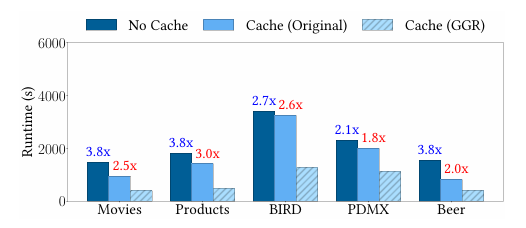
\includegraphics[width=\linewidth]{Images/Filter Queries.png}
\caption{Filter Queries}
\label{fig:Filter Queries}
\end{subfigure}
\begin{subfigure}[b]{0.4\linewidth}
\centering
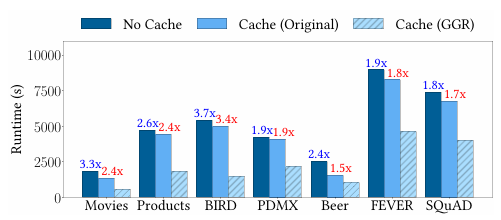
\includegraphics[width=\linewidth]{Images/RAG Queries.png}
\caption{RAG Queries}
\label{fig:RAG Queries}
\end{subfigure}
\caption{ End-to-end Result (Filter, Selection, RAG): Our optimizations Cache (GGR) achieve 1.5– 3.4× speed-up in end-to-end runtime
over caching without reordering (Cache (Original)), and 1.8– 3.8× over No Cache baseline.}
\label{fig:filter and RAG}
\end{figure}
\textbf{LLM filter}. We find that filter queries, which tend to produce short outputs like "Yes/No" or sentiment labels, benefit the most from caching: Cache (GGR) achieves 2.1–3.8× speedup over No Cache, while plain caching without reordering only gets a modest 1.03–1.9× boost. We attribute this gap directly to our reordering — GGR further cuts latency by 1.8–3.0× over Cache (Original) by rearranging rows and fields to maximize how much of each prompt's prefix can be reused.
Most of our review-style datasets — Movies, Products, and BIRD — start out with highly unique fields (like review content) due to how they're joined with metadata tables, which hurts caching by default. We show that reprioritizing fields with more repeated values, like description or product title, raises prefix hit rates by 57–74~\%\ and gives us a 2.5–3× speedup. We highlight PDMX as a harder case, since its 57 fields are mostly long and unique, so even though we boost its hit rate from 12~\%\ to 57~\%\, we only get a 1.8× speedup because 43~\%\ of requests still miss the cache. Beer, by contrast, already has some natural duplication, so GGR pushes its hit rate from 50~\%\ to 80~\%\ for a 2× speedup.
\textbf{LLM projection}. We test this on longer-output tasks like summarization and find Cache (GGR) achieves 2.4–3.7× speedup over No Cache and 1.5–3.4× over Cache (Original). We note that as output length grows, the decode stage starts to dominate runtime, which shrinks the relative benefit of prefill caching compared to filter queries — except on datasets like BIRD and PDMX, where long strings mean caching also saves meaningful memory during decoding.
\begin{figure}[h]
  \centering
  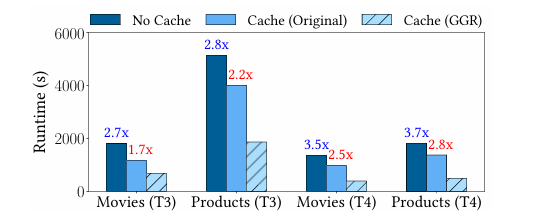
\includegraphics[width=0.8\textwidth]{Images/Aggregation.png}
  \caption{ End-to-end Result (Multi-LLM Invocation, Aggrega
tion): Our optimizations Cache (GGR) achieve 1.7- 2.8× speed-up over Cache (Original), and 2.7- 3.7× speed-up over No Cache.}
  \label{fig:Aggregation}
\end{figure}
\textbf{Multi-LLM invocation}. We combine a filter step with a projection step and find Cache (GGR) achieves 2.7–2.8× speedup over No Cache and 1.7–2.2× over Cache (Original). We explain that this relative gain is smaller than for single-step queries because the first (filter) invocation runs over already-distinct reviews, so caching and reordering don't help as much there — the benefit mostly comes from wherever the second invocation dominates runtime.
\textbf{LLM aggregation}. We use an AVG operator over LLM-generated sentiment scores and see 3.5–3.7× speedup over No Cache and 2.5–2.8× over Cache (Original), results we describe as closely mirroring the filter-query numbers since output lengths are similarly short.
\begin{table}[h]
\centering
\begin{tabular}{lccccccc}
\toprule
Method & Movies & Prods. & BIRD & PDMX & Beer & FEVER & SQuAD \\
\midrule
\textbf{Original} & 35\% & 27\% & 10\% & 12\% & 50\% & 11\% & 11\% \\
\textbf{GGR} & 86\% & 83\% & 85\% & 57\% & 80\% & 67\% & 70\% \\
\bottomrule
\end{tabular}
\caption{PHR (\%) of LLM Filter and RAG queries for Original and
GGR, which achieves 30 -- 75\% higher hit rates.}
\label{tab:phr}
\end{table}
\textbf{RAG}. We evaluate this on FEVER and SQuAD, retrieving supporting contexts via vector search before answering, and find Cache (GGR) achieves 1.9× speedup over No Cache and 1.7–1.8× over Cache (Original). We attribute this to GGR's ability to rearrange overlapping contexts across questions, boosting prefix hit rate by 56–59~\%\ over the unreordered baseline.
\begin{figure}[h]
  \centering
  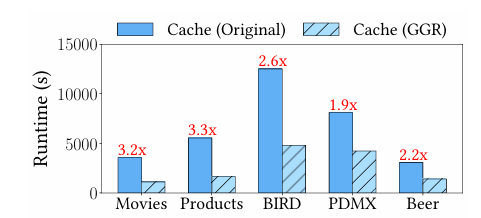
\includegraphics[width=0.8\textwidth]{Images/Cache.png}
  \caption{ Cache(GGR)isabletoachieve1.9–3.3×speed-upover
Cache(Original)forfilterqueriesonLlama3-70B.}
  \label{fig:Cache}
\end{figure}
Results on the larger Llama-3-70B model, run across 8 L4 GPUs, show a similar pattern — Cache (GGR) achieves 1.9–3.3× speedup over Cache (Original), confirming our approach's benefits hold as model size scales up.
\subsection{Cost Savings on Proprietary API Endpoints}
We test our GGR reordering against real OpenAI~\cite{openai_pricing} and Anthropic~\cite{anthropic_prompt_caching} pricing, since both offer discounts for cached tokens. Because both providers require a minimum 1,024-token prefix to cache at all, we duplicate FEVER's fields to simulate a more realistic long-input dataset. We find GGR delivers 32~\%\ cost savings on GPT-4o-mini and 21~\%\ on Claude 3.5 Sonnet, while the original ordering gets 0~\%\ cache hits since its prefixes never meet the minimum threshold. Extrapolating from our earlier hit-rate measurements across all seven datasets, we estimate GGR could yield 20–39~\%\ savings under OpenAI's pricing and up to 79~\%\ under Anthropic's, assuming future support for arbitrary-length prefix caching.
\begin{table}[h]
\centering
\begin{tabular}{llllll}
\toprule
Dataset & Model & Method & PHR (\%) & Cost (\$) & Savings (\%) \\
\midrule
\multirow{4}{*}{FEVER}
 & \multirow{2}{*}{4o-mini} & Original & 0.0  & 0.81 & -- \\
 &                          & GGR      & 62.2 & 0.55 & 32\% \\
 & \multirow{2}{*}{Sonnet}  & Original & 0.0  & 5.49 & -- \\
 &                          & GGR      & 30.6 & 4.33 & 21\% \\
\bottomrule
\end{tabular}
\caption{OpenAI and Anthropic Costs: cache hit rate (HR\%), cost,
and savings comparison of GGR over Original for GPT-4o-mini
and Claude 3.5 Sonnet in FEVER.}
\label{tab:openai-anthropic-costs}
\end{table}
\begin{table}[H]
\centering
\begin{tabular}{lccccc}
\toprule
\multirow{2}{*}{Dataset} & \multicolumn{2}{c}{PHR (\%)} & \multicolumn{2}{c}{Est. Cost Savings (\%)} \\
\cmidrule(lr){2-3} \cmidrule(lr){4-5}
 & Original & GGR & OpenAI & Anthropic \\
\midrule
Movies   & 34.6 & 85.7 & 31 & 73 \\
Products & 26.7 & 83.3 & 33 & 73 \\
BIRD     & 10.4 & 84.8 & 39 & 79 \\
PDMX     & 11.8 & 56.6 & 24 & 48 \\
Beer     & 49.9 & 80.1 & 20 & 55 \\
FEVER    & 11.2 & 67.4 & 30 & 60 \\
SQuAD    & 11.0 & 69.7 & 31 & 63 \\
\bottomrule
\end{tabular}
\caption{Estimated cost savings: across datasets using PHR from
Sec 6.2 and OpenAI and Anthropic's pricing model.}
\label{tab:estimated-cost-savings}
\end{table}
\subsection{Impact of Reorder ingon Accuracy}
Since GGR changes the order fields appear in the prompt, we check whether that hurts model accuracy on LLM filter queries and one RAG query (FEVER), using bootstrapped accuracy distributions across 10K runs on Llama-3-8B, Llama-3-70B, and GPT-4o. We find GGR's accuracy stays within about 5~\%\ of the original ordering in almost every case — the one notable exception is FEVER with Llama-3-8B, where GGR actually improves accuracy by 14.2~\%\, because it happens to place the "claim" field at the end of the prompt, which that particular model prefers. We note this effect doesn't hold for the larger models, and overall conclude that bigger models like Llama-3-70B and GPT-4o are more robust to field reordering.
\begin{figure}[!htbp]
\centering
\begin{subfigure}[b]{0.32\linewidth}
\centering
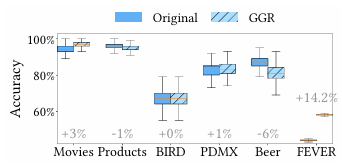
\includegraphics[width=\linewidth]{Images/8B.png}
\caption{Meta-Llama-3-8B-Instruct}
\label{fig:8B}
\end{subfigure}
\begin{subfigure}[b]{0.32\linewidth}
\centering
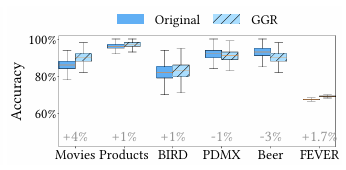
\includegraphics[width=\linewidth]{Images/70B.png}
\caption{Meta-Llama-3-70B-Instruct}
\label{fig:70B}
\end{subfigure}
\begin{subfigure}[b]{0.32\linewidth}
\centering
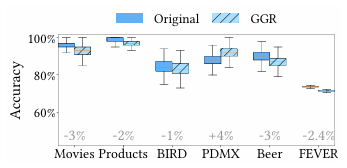
\includegraphics[width=\linewidth]{Images/openAPI.png}
\caption{OpenAIGPT-4o}
\label{fig:openAPI}
\end{subfigure}
\caption{Accuracy of original v.s.GGR ordering:we perform statistical bootstrapping to get a distribution of exact match accuracy
measurements across 10,000runs.The numbers indicate the difference in the median accuracy of GGR compared to the original ordering..}
\label{fig:Accuracy}
\end{figure}
\subsection{Algorithm Overhead}
We check whether GGR's own runtime eats into the speedups it provides, looking separately at latency and memory. On latency, we find GGR consistently finishes in under 15 seconds across all our datasets — even ones with up to 30K rows and 57 fields — which works out to less than 0.01~\%\ of total LLM query runtime, so the reordering overhead is effectively negligible. On memory, we note that GGR only ever needs the specific table touched by the query loaded into memory, and since its recursive splitting keeps shrinking the table at each step, total memory usage stays at O(n×m), with just minor additional overhead from the recursion stack and temporary variables.
\section{RELATED WORK}
\label{sec:related-work}
Our optimizations build on recent work in LLM inference as well as prior work integrating machine learning and data management.

\textbf{Inference-optimized systems.} There has been a recent rise of dedicated systems for LLM inference, including FasterTransformer~\cite{nvidia2023fastertransformer}, Orca~\cite{yu2022orca}, vLLM~\cite{kwon2023vllm}, and SGLang~\cite{zheng2023sglang}. Many of these systems already explore memory-efficient GPU kernels that perform inference while leveraging shared prefixes — SGLang's RadixAttention~\cite{zheng2023sglang}, Hydragen~\cite{juravsky2024hydragen}, and Cascade Inference~\cite{ye2024cascade} all implement optimized kernels along these lines. Our work builds upon this prior work on high-throughput LLM inference and prefix caching for model serving, and additionally leverages full workload information from batch queries to further improve performance in relational workloads.

\textbf{LLMs in relational data analytics.} Many systems support calling LLMs as operators on relational data, spanning from production database vendors like Databricks~\cite{databricks_ai_functions}, Google BigQuery~\cite{bigquery_llm}, and AWS Redshift~\cite{aws_redshift_llm} to programming frameworks like LOTUS~\cite{patel2024lotus}. While these works provide APIs for running LLMs over relational data, they do not explore how reordering data can optimize KV cache hits. There is also a line of work~\cite{kang2017noscope,lu2018probabilistic} that explores using cheaper models for approximate query generation; this orthogonal direction is not considered in our paper's scope, as our work specifically focuses on calling LLMs as functions from inside a regular, given SQL query.
\section{CONCLUSION}
In this paper,we introduce techniques to optimize LLM in 
vocations in relational data analytics workloads.By leverag
ing workload information coupled with observations about 
the LLM inference process,we can significantly improve 
end-to-end query performance and reduce costs without af
fecting query semantics.Our technique achieves upto 3.4× 
decreases in end-to-end query latency with Llama-3-8B and 
Llama-3-70B and also achieves upto 32\%\ cost savings 
under OpenAI and Anthropic pricing models.
\begin{acks}
We thank Soujanya Ponnapalli for helpful discussions and feedback, 
and Jelani Nelson for academic advising. This research was supported 
by gifts from Accenture, AMD, Anyscale, Broadcom Inc., Google, IBM, 
Intel, Intesa San Paolo, Lambda, Mibura Inc., Samsung SDS, and SAP.
\end{acks}
\bibliographystyle{ACM-Reference-Format}
\bibliography{biblio}
\end{document}